\section{Solution Methods of RL}\label{Solution Methods}
The solution methods for the reinforcement learning problem can be divided into two groups, \textit{tabular} and \textit{approximate}. The tabular solution methods find exact, optimal solutions and are more suitable when the states and actions space is rather small, while the approximate solution methods provide approximate solutions and it is applicable to large spaces problems.

The process of \textit{generalized policy iteration} (GPI) provides a good way of getting insight into the methods of RL. GPI employs a sequence of interleaved policy evaluations and policy improvements, where the given policy is evaluated, for example, by computing it's value function, and the policy is improved by using the value function. This process is proven to converge to an optimal policy and value function for the classical dynamic programming methods. GPI represents the way that almost all RL methods work. The \Cref{fig:GPI} illustrates the process better.
\begin{figure}[H]
	\centering
	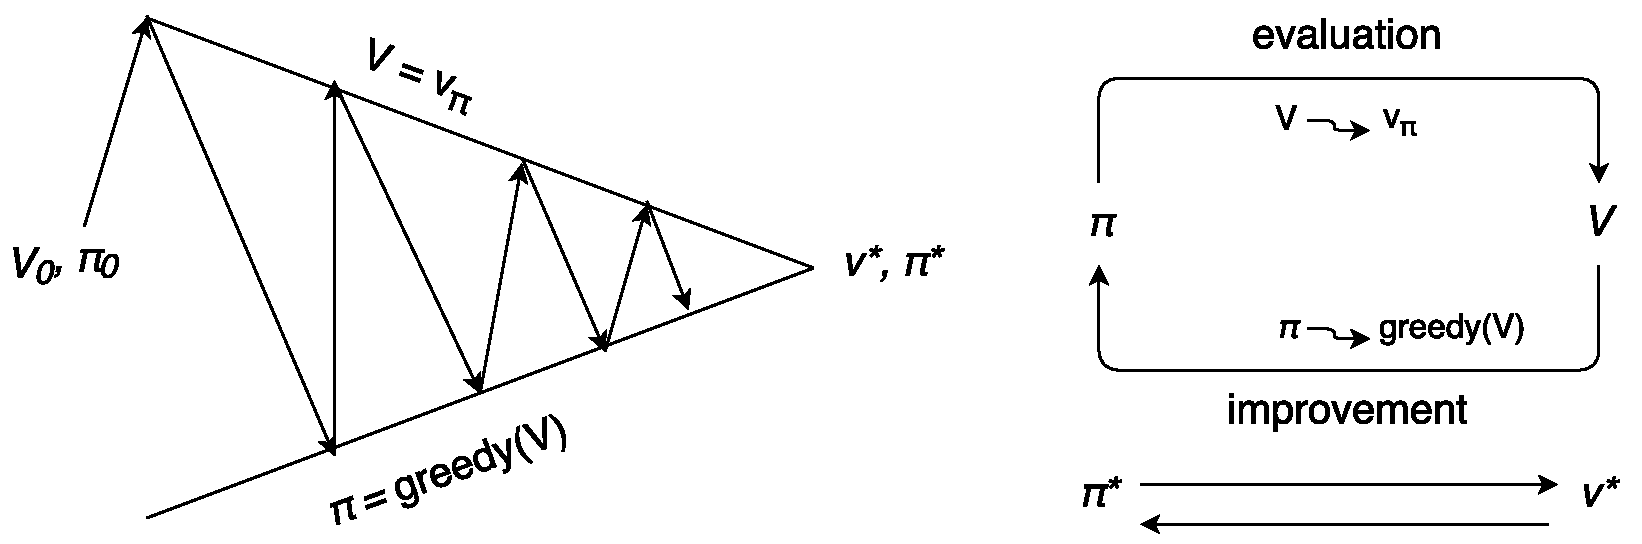
\includegraphics[width=0.9\textwidth]{Figures/GPI}
	\caption{Generalized Policy Iteration}
	\label{fig:GPI}
\end{figure}
Another way of presenting the GPI is in terms of \textit{prediction} and \textit{control}. The prediction problem is referring to policy evaluation or the estimation of $v_{\pi}$ for a given policy $\pi$, whereas the control problem is referring to the actual optimal policy $\pi_{*}$ seeking.

The relevant notions for describing the methods of RL are \textit{backup} and \textit{bootstrap}. A \textit{full backup} updates a state's value on the basis of the next states estimated values. \textit{Bootstrapping} refers to the idea of updating estimates based on other estimates.

Usually, the RL solution methods vary in the way they approach the prediction and control problems, and also in whether they need a model of the environment or they use bootstrapping.

\subsection{Tabular Solution Methods}
The tabular solution methods include three important classes of methods for solving the finite MDP: \textit{Dynamic Programming} (DP), \textit{Monte Carlo} (MC) and \textit{Temporal-Difference} (TD) learning. These methods will be generally presented in the following pages.

\subsubsection{Dynamic Programming}
Dynamic programming uses the Bellman optimality equations \ref{BellmanOptimalityVstar} and \ref{BellmanOptimalityQstar} as update functions for \textit{policy iteration}, which yields a sequence of monotonically increasing value functions and policies: ${\pi}_{0}\overset{E}{\rightarrow}v_{{\pi}_{0}}\overset{I}{\rightarrow}{\pi}_{1}\overset{E}{\rightarrow}v_{{\pi}_{1}}\overset{I}{\rightarrow}{\pi}_{2}\overset{E}{\rightarrow}...\overset{I}{\rightarrow}{\pi}_{*}\overset{E}{\rightarrow}v_{*}$, where $E$ stands for evaluation and $I$ - for improvement. That is, an arbitrary fixed policy is evaluated by computing it's state-value function and is improved by computing it's state-action value function. If the state-action value function of choosing an action $a \neq \pi(s)$ is greater than the state-value function $v_{\pi}(s)$, then the policy is changed to a new policy. The formula for getting a new policy is given by \ref{PolicyImprovement}:
\begin{equation}\label{PolicyImprovement}
\begin{split}
\pi'&=\arg\!\max_{a}q_{\pi}(s,a)\\
&=\arg\!\max_{a}\mathop{{}\mathbb{E}}\left [ R_{t+1} + \gamma v_{\pi}(S_{t+1})|S_{t}=s, A_{t}=a  \right ] \\
&=\arg\!\max_{a}\sum_{s',r}p(s',r|s,a)\left [ r+\gamma v_{\pi}(s') \right ]
\end{split}
\end{equation}

Unlike the DP methods, the Monte Carlo and the temporal-difference solution methods don't require the model parameters to be known in advance, meaning that no previous knowledge about the environment is needed and that the agent learns exclusively from it's \textit{experience} (sampled states, actions, rewards). The MC method doesn't bootstrap, whereas TD does use bootstrapping, like the DP methods.

\subsubsection{Monte Carlo}
Monte Carlo differs from DP in the way it handles the prediction problem. It uses averages over the sampled returns from a specific state on episode-by-episode basis in order to learn over multiple observed returns the value function, whereas in DP the value function was computed from the knowledge of the MDP. The policy evaluation is performed by computing the value of the state-action pairs for the visited states over an episode. The policy improvement is performed by adjusting the policy closer to the action with the maximal value for a specific state.

Because MC doesn't make all the possible actions, it is required to employ some kind of guarantee for exploration. This can be achieved by assigning nonzero probabilities for all the actions in order to make sure they are going to be picked eventually. This is called \textit{exploring starts}. A better approach are the \textit{on-policy} and \textit{off-policy} methods. 

On-policy methods have probabilities greater than zero for all their actions, meaning that they have \textit{soft} policies. The policies in on-policy methods become closer to an optimal deterministic policy in time. The exploring starts is an example of on-policy method. Another example would be an $\epsilon$-greedy policy where the best action is chosen with the probability $1-\epsilon$ and, sometimes, another random action is chosen with the probability $\epsilon$.

Off-policy methods use 2 policies: a \textit{target policy} $\pi$, which is a deterministic policy, like the one presented in the on-policy methods, and a \textit{behavior policy} $\mu$, which is stochastic in states and generates data by exploring. Both policies have non zero probabilities that ensures the coverage property. Off-policy methods can be implemented with \textit{importance sampling} technique. The importance sampling technique computes an importance sampling ratio based on the relative probabilities of the returns' trajectories from both policies and it is used for weighting the returns for learning the value function.

\subsubsection{Temporal Difference}\label{Temporal Difference}
Temporal Difference differs from DP also in the way it handles the prediction problem. TD makes an estimate of the value function after each time step by sampling expected values and using current value estimates. Therefore, TD is a combination of MC sampling and DP bootstrapping. The simplest TD method is also called \textit{TD(0)}. The update function for TD(0) \ref{PolicyEvaluationTD0} is the following:
\begin{equation}\label{PolicyEvaluationTD0}
V(S_{t})\leftarrow V(S_{t})+\alpha \left [ R_{t+1}+\gamma V(S_{t+1})-V(S_{t}) \right ]
\end{equation}
If we compare the MC target with the TD target, the MC target has $G_{t}$ instead of the immediate reward and the value estimate of the next state. The square brackets represents the TD error, or the MC error in the MC update function. An important observation is that the sum of the time steps TD errors gives an episode of MC error.

For solving the control problem with TD(0) and on-policy methods, action-value functions are used instead of the value function that we've just seen. A "transition from one action-state pair to another" \cite{Sutton} yields a quintuple of the form $(S_{t}, A_{t}, R_{t+1}, S_{t+1}, A_{t+1})$, \textit{Sarsa}, which is the name of the algorithm. Therefore, for evaluating the policy, an estimation of the $q_{\pi}$ is required and for improving the policy, $\pi$ is greedily adjusted closer to it's $q_{\pi}$.

An notable off-policy TD(0) algorithm is \textit{Q-learning}. It is an off-policy method because it learns the optimal action-value function $q_{\pi*}$ independent of the policy. The action is picked greedily according to the estimated $Q$ but the $Q$ is updated based on the action that produces maximal value. 

A slight change into the update function of $Q$ would lead us to the \textit{Expected Sarsa} algorithm. The change is that instead of maximizing over the next action-value pairs, the expected return is taken, which considers the probabilities of making those actions according to the current policy. Expected Sarsa is a better algorithm in comparison with Sarsa and Q-learning.

The MC and TD methods are extended into more complicated and powerful forms to achieve better performance, but the essence of these methods perpetuates in all the other algorithms. An idea about combining these two methods would be to unify them under \textit{n-step} algorithms instead of the extreme one time step in TD(0) and a whole episode in MC, or perform additions of other features like eligibility traces and model learning.
	
\subsection{Approximate Solution Methods}\label{Approximate solution methods}
The approximate solution methods are an extension to the tabular solution methods for huge states spaces problems. In this type of problems, the goal is to find a good approximate solution under the condition of restricted computational resources. Because almost every visited state is seen for the first time, every state being so unique, the agent needs to be able to make sense of it and, therefore, usefully generalize the information it gets. This is possible thanks to function approximation. “Function approximation is an instance of supervised learning, the primary topic studied in machine learning, artificial neural networks, pattern recognition, and statistical curve fitting” \cite{Sutton}.

The value function is represented by a function of a weights vector instead of a table. The approximated value function looks like $\hat{v}(s,\theta)\approx v_{\pi}(s)$, which can be translated into words as the approximated value of a state $s$ given the weights vector $\theta$. The value function can be an artificial neural network with multiple layers where the weights are adjusted and learned. A single adjustment of the weights would change the value appreciation for all the states. This process is difficult to follow and track, but it is more powerful. This would create the necessary \textit{generalization} for the agent to learn from it and apply knowledge in multiple similar, but different states.

With function approximation different supervised machine learning methods can be applied to simulate outputs for a set of inputs. The estimated value of a state $s$ should look more like a number $g$ and this relation $s \mapsto g$ can be used as a training example for supervised learning that would learn to predict values for other states. $s \mapsto g$ is referred to as a back-up, where $s$ is the state backed-up and $g$ is the backed-up value or target. For example, the target in MC methods is the return $G_{t}$, so the back-up is $S_{t} \mapsto G_{t}$, whereas the back-up in TD(0) is $S_{t} \mapsto R_{t+1}+\gamma\hat{v}(S_{t+1}, \theta_{t}) $.

Some common way of doing function approximation is based on gradient principles. For any $\theta$ the function approximator can not exactly represent all the states and examples, therefore the idea is to find a balance - a weights vector that would, as close as possible, represent all the states. A performance measure could be defined by the \textit{mean squared value error} (MSVE) shown below (\Cref{MSVE}). The error represents the squared difference between the estimated value $\hat{v}(s,\theta)$ and the actual value $v_{\pi}(s)$, whereas the $d(s)$ represents the weight or the distribution of the error for a state $s$. The goal would become the minimization of MVSE.
\begin{equation}\label{MSVE}
MVSE(\theta)=\sum_{s\in S} d(s) \left [ v_{\pi}(s) - \hat{v}(s,\theta) \right ]^{2}
\end{equation}

For each training example the \textit{Stochastic Gradient Descent} (SGD) method would update the weights so that they minimize the error in that example:
\begin{equation}\label{SGD}
\theta_{t+1}=\theta_{t}+\alpha \left [ v_{\pi}(S_{t}) - \hat{v}(S_{t},\theta_{t}) \right ]\nabla\hat{v}(S_{t},\theta_{t})
\end{equation}
In the MC method, the target is an unbiased estimate of $v_{\pi}(s)$, therefore the SGD would be a good choice to be applied, because it would converge to a locally optimal solution for the value function. In the bootstrapping cases, however, SGD is not the best choice, because the targets usually depend on the weights vector that is changing and causing the targets to be biased. These methods are called \textit{semi-gradient} methods instead, and they converge in the linear case.

Linear methods have feature vectors $\phi(s)$ that represent the state. The inner product between the feature vector $\phi(s)$ and the weights $\theta$ makes up the function approximation $v_{\pi}(s,\theta)$. In such a situation the SGD method can be applied and get an even simpler form of weights update. This is proven to converge to a global optimum, including for the MC linear function approximation version and the semi-gradient TD(0) with an additional theorem.

\subsubsection{Policy Gradient Methods} \label{PolicyGradMeths}
The \textit{Policy Gradient Methods} learn a \textit{parameterized policy} and makes it possible to select the action without calculating the value function. So, in a given state $s$, at a given time $t$, the agent selects an action $a$ based on the weights vector ${\theta}$ of the policy: ${\pi}(a|s,{\theta})=Pr\{A_{t}=a|S_{t}=s,{\theta}_{t}={\theta}\}$. The policy weights are learned according to an approximate gradient of a performance indicator ${\eta}({\theta})$ with respect to the policy weights, which tries to maximize the performance. All the methods of the form \Cref{gradM} are policy gradient methods:
\begin{equation}\label{gradM}
\theta_{t+1}=\theta_{t}+\alpha \nabla \eta (\theta_{t})
\end{equation}

The policy gradient methods are suitable for both \textit{discrete} and \textit{continuous} action spaces. For the discrete action space problems parameterized numerical preferences can be formed for each state-action pair, $h(s,a,\theta)$ \cite{Sutton}. The most preferred actions in each state have the highest probability of getting selected. The preferences can be parameterized randomly, for example, by being computed by a deep Q-network. The policy gradient theorem provides a formula for computing the gradient of the performance measure $\eta$ with respect to the policy weights vector $\theta$, composed of the state distribution $d_{\pi}(s)$, the state-action value function $q_{\pi}(s,a)$, and the gradient of the policy $\nabla_{\theta}\pi(a|s,\theta)$:
\begin{equation}\label{gradMTheorem}
\nabla\eta(\theta)=\sum_{a}d_{\pi}(s)\sum_{a}q_{\pi}(s,a)\nabla_{\theta}\pi(a|s,\theta)
\end{equation}

The methods that use both policy and value approximations are named \textit{actor-critic} methods, where the \textit{actor} estimates the policy weights vector for choosing an action and the \textit{critic} estimates the value weights for providing the information about the quality of a state the agent ends up in after making the action according to the policy. So, the actor is about the learned policy, and the critic - about the learned value function. 

There is an algorithm which is called \textit{reinforce} and it also uses both policy and value function approximation, but it doesn't bootstrap. The critic, on the other hand, is a bootstrapping critic, which updates it's states based on the value estimates of the next states. So, the initial reinforce algorithm has been changed for the actor-critic method: it's full return was replaced by one-step return. The one-step actor critic algorithm is presented below \cite{Sutton}.
\begin{algorithm}[H]
	\caption{One-step Actor-Critic (episodic)}
	\label{algo:AC}
	\begin{algorithmic}
		\State Input: differentiable policy parameterization $\pi(a|s,\theta),\forall a\in A, s\in S,\theta\in\mathbb{R}^{n}$
		\State Input: differentiable state-value parameterization $\hat{v}(s,w),\forall s \in S, w \in \mathbb{R}_{m}$
		\State Parameters: $\alpha>0,\beta>0$
		\State Initialize policy weights $\theta$ and state-value weights $w$
		\Repeat
		\State Initialize $S$ (first state of episode)
		\State $I\leftarrow 1$
		\While{$S$ is not terminal}:
		\State $A\sim \pi(\cdot|S,\theta)$
		\State Take action $S$, observe $S'$, $R$
		\State $\delta\leftarrow R+\gamma\hat{v}(S',w)-\hat{v}(S,w)$ (if $S'$ is terminal, then $\hat{v}(S',w)=0$)
		\State $w\leftarrow w+\beta\delta\nabla_{w}\hat{v}(S,w)$
		\State $\theta\leftarrow \theta+\alpha I \delta\nabla_{\theta} \textup{log} \pi(A|S,\theta)$
		\State $I\leftarrow \gamma I$
		\State $S\leftarrow S'$
		\EndWhile
		\Until forever
	\end{algorithmic}
\end{algorithm}

As it was mentioned before, policy gradient methods work for discrete action spaces as well as for continuous. In the discrete actions problem, the policy is estimating the probability of each action in the discrete set. In the continuous actions space, on the other hand, the policy approximates the variance $\sigma^2$, and the mean $\mu$ of a normal distribution given by:
\begin{equation}\label{normalDistrib}
p(x)=\frac{1}{\sigma \sqrt{2\pi}}\textup{exp}(-\frac{(x-\mu)^2}{2\sigma ^2}),
\end{equation}
where $p(s)$ is the density of the probability at $x$. This is what makes the basis for the construction of a continuous policy, in which the weights-vector $\theta$ is included. The continuous policy formula is provided below:
\begin{equation}\label{continuousPolicy}
\pi(a|s,\theta)=\frac{1}{\sigma (s,\theta) \sqrt{2\pi}}\textup{exp}(-\frac{(a-\mu(s,\theta))^2}{2\sigma(s,\theta) ^2})
\end{equation}
The policy weights vector $\theta=[\theta_{\mu}, \theta_{\sigma}]^T$ is composed of two elements, $\theta_{\mu}$ and $\theta_{\sigma}$, that can be used further in function approximation algorithms. The form that these elements take is shown below:
\begin{equation}\label{mean}
\mu(s,\theta) = \theta_{\mu}^T\phi(s) \textup{    and    }
\sigma(s,\theta) = \textup{exp} (\theta_{\sigma}^T\phi(s)),
\end{equation}
where $\phi(s)$ is the feature vector, which can be, for example, the pixel values vector of an image.